% Created 2012-03-28 Wed 12:30
\documentclass[a4paper]{article}
\usepackage[utf8]{inputenc}
\usepackage[T1]{fontenc}
\usepackage{fixltx2e}
\usepackage{graphicx}
\usepackage{longtable}
\usepackage{float}
\usepackage{wrapfig}
\usepackage{soul}
\usepackage{textcomp}
\usepackage{marvosym}
\usepackage{wasysym}
\usepackage{latexsym}
\usepackage{amssymb}
\usepackage{hyperref}
\tolerance=1000
\usepackage{verbatim}
\setlength{\parindent}{0in}
\providecommand{\alert}[1]{\textbf{#1}}

\title{Public Health Surveillance Shortcourse \\GIS for surveillance}
\author{Ivan Hanigan}
\date{\today}
\hypersetup{
  pdfkeywords={},
  pdfsubject={},
  pdfcreator={Emacs Org-mode version 7.8.03}}

\begin{document}

\maketitle

\setcounter{tocdepth}{3}
\tableofcontents
\vspace*{1cm}
\hrule

\section{Background}
\label{sec-1}

In this demonstration we'll use the online working paper by Glynn (2011) at \href{http://www.franklincenterhq.org/2541/geocoding-addresses-from-missouri-sex-offender-registry/}{http://www.franklincenterhq.org/2541/geocoding-addresses-from-missouri-sex-offender-registry/}
\cite{Glynn2011} and \cite{Glynn} to call Google's Geocoding API
\cite{Google} for a set of example individuals given their street,
city and state.  The example data are sourced from the Missouri Sex
Offender Registry. For further information see the `Action News'
article \cite{Kath2011} or the Economist \cite{TheEconomi2009}.
\section{R codes}
\label{sec-2}

The worked example does the data manipulations using the R statistical
analysis language \href{http://www.r-project.org/}{http://www.r-project.org/}. Download the R files from
the website \href{http://dl.dropbox.com/u/7075452/PHsurveillance_overview.org}{http://dl.dropbox.com/u/7075452/PHsurveillance\_overview.org} and store in a working directory. 
\begin{comment}
 I used the package
ProjectTemplate to set up a directory called `analysis' which
automatically creates a `src' directory for source code files and a
`data' directory for data files.  The other directories are included
by default and have more esoteric functions that we will not use in
this example.
\end{comment}
\section{Download example data}
\label{sec-3}

The source of the data is at the bottom of this website \\ 
\href{http://www.mshp.dps.mo.gov/MSHPWeb/PatrolDivisions/CRID/SOR/SORPage.html}{http://www.mshp.dps.mo.gov/MSHPWeb/PatrolDivisions/CRID/SOR/SORPage.html}
\section{Load and clean}
\label{sec-4}

Glynn has provided a downloadable source code file for cleaning the
data.  All we need to do manually is to open the Excel file and delete
the top 13 lines of summary information, after that deletion we saved
the data to a new Excel file named Missouri-Sex-Offenders.xls.  R
would now read this file.
\section{Do geocoding}
\label{sec-5}

This step takes some time.  There is also the issue that Google restricts users to only geocoding 2500 addresses per day.  Therefore the full 12174 addresses would take 4.9 days to complete.
\section{Check outputs}
\label{sec-6}




An estimate of the precision of the geocode is given in the location\_type feild.  This stores additional data about the specified location. The following values are currently supported:
\begin{itemize}
\item ROOFTOP indicates that the returned result is a precise geocode for which we have location information accurate down to street address precision.
\item RANGE\_INTERPOLATED indicates that the returned result reflects an approximation (usually on a road) interpolated between two precise points (such as intersections). 
\item GEOMETRIC\_CENTER indicates that the returned result is the geometric center of a result such as a polyline (for example, a street) or polygon (region).
\item APPROXIMATE indicates that the returned result is approximate.
\end{itemize}
\section{Find a specific offender}
\label{sec-7}

From the article in the Economist \cite{TheEconomi2009} we know that Janet Allison was found guilty because she let her 15-year-old daughter have sex with a boyfriend she later married. But Ms Allison will ``spend the rest of her life publicly branded as a sex offender.'' So let's look her up.




\begin{center}
\begin{tabular}{lll}
 ALLISON, CORD J     &  3655 PENNRIDGE DR APT 220  &  CHILD MOLEST-2ND DEGREE                    \\
 ALLISON, EARNEST E  &  2737 US HWY 65             &  DEVIATE SEXUAL ASSAULT                     \\
 ALLISON, JOE E      &  22123 AUDRAIN RD 9318      &  POSSESSION OF CHILD PORNOGRAPHY            \\
 ALLISON, STEVEN L   &  10390 HWY D                &  ENDANGERING WELFARE OF A CHILD-1ST DEGREE  \\
 HOPSON, ALLISON M   &  4258 ST LOUIS AVE          &  RAPE                                       \\
\end{tabular}
\end{center}



This person does not live in Missouri, but in Georgia.
\section{Put somebody on the map}
\label{sec-8}




\begin{center}
\begin{tabular}{lll}
 AARON, JEFFERY W  &  371 YEARGAN LN  &  SEXUAL ABUSE IN THE SECOND  \\
\end{tabular}
\end{center}




\begin{figure}[!h]
\centering
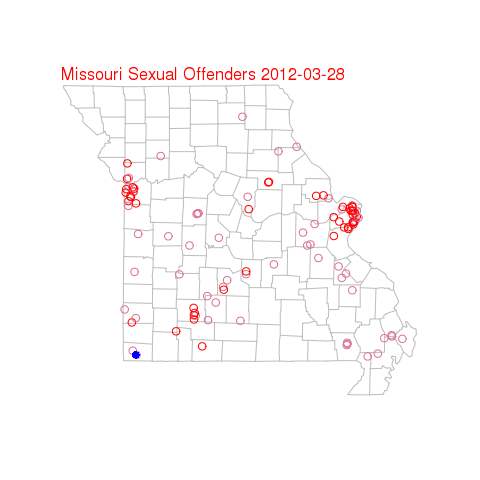
\includegraphics[width=\textwidth]{offenderIdentified.png}
\caption{offenderIdentified.png}
\label{fig:offenderIdentified.png}
\end{figure}
\clearpage
\section{Write the final(ish) data}
\label{sec-9}

To facilitate using the data in a GIS package we'll write these points out to a ESRI Shapefile.  The Shapefile is probably the most common format you find spatial data in; as Wikipedia points out it is `a (mostly) open specification for data interoperability among GIS software'.  The code also shows how to easily re-project the data into arbritrary coordinate systems (sometimes important for getting multiple data sources to relate) and we'll go for WGS84 as it is also common. 
\section{Next steps}
\label{sec-10}

The worked examples on this website continue through the steps required to set up an interactive web map so that the surveillance system can be utilised by the general public \\
\href{http://batchgeo.com/map/356612ae67bb92de8c91dd9fb7e27029}{http://batchgeo.com/map/356612ae67bb92de8c91dd9fb7e27029}.  
\section{References}
\label{sec-11}

\begin{comment}
\bibliographystyle{unsrt}
\bibliography{I:/references/library}
\end{comment}

\begin{thebibliography}{1}

\bibitem{Glynn2011}
Earl~F Glynn.
\newblock {Geocoding addresses from Missouri Sex Offender Registry: Computer
  Assisted Reporting.
  [[http://www.franklincenterhq.org/2541/geocoding-addresses-from-missouri-sex-offender-registry/][http://www.franklincenterhq.org/2541/geocoding-addresses-from-missouri-sex-offender-registry/]]}.
\newblock Technical report, Franklin Center for Government and Public
  Integrity, Bismarck, ND, 2011.

\bibitem{Glynn}
Earl~F Glynn.
\newblock {GoogleGeocode.R,
  [[http://cdn.watchdogmedia.org/national/computer-assisted-reporting/project/geocoding-and-distances/missouri-sex-offenders/GoogleGeocode.R][http://cdn.watchdogmedia.org/national/computer-assisted-reporting/project/geocoding-and-distances/missouri-sex-offenders/GoogleGeocode.R]]}, 2010.

\bibitem{Google}
Google.
\newblock {Google Geocoding API,

  [[http://code.google.com/apis/maps/documentation/geocoding/index.html][http://code.google.com/apis/maps/documentation/geocoding/index.html]]}.

\bibitem{Kath2011}
Ryan Kath.
\newblock {Loophole in law allows hundreds of Missouri sex offenders to live
  near church day cares,
  [[http://www.kshb.com/dpp/news/local\_news/investigations/loophole-in-law-allows-hundreds-of-missouri-sex-offenders-to-live-near-church-daycares][http://www.kshb.com/dpp/news/local\_news/investigations/loophole-in-law-allows-hundreds-of-missouri-sex-offenders-to-live-near-church-daycares]]}.
\newblock {\em KSHB NBC Action News}, 2011.

\bibitem{TheEconomi2009}
The Economist.
\newblock {America's unjust sex laws,
  [[http://www.economist.com/node/14165460?story\_id=14165460][http://www.economist.com/node/14165460?story\_id=14165460]]}.
\newblock {\em The Economist}, 2009.

\end{thebibliography}

\end{document}
